\section{Globaal ontwerp}  \label{sec:globaal}
Canvas.hs is een library die de programmeur kan importeren in zijn programma om er daarna met de API die Canvas.hs aanbiedt gemakkelijk een uitgebreide user interface mee te bouwen. Canvas.hs focust zich op elementaire input en heeft geen ondersteuning heeft voor high level interface elementen zoals knoppen en textgebeiden. Deze elementen zijn met behulp van Canvas.hs gemakklijk te implementeren. \autoref{fig:demo_screenshot} geeft een demoapplicatie van Canvas.hs weer.

\todo{hier uitwijden over principe van Canvas.hs? Als het goed is al in inleiding gebeurd. Moet iig verteld zijn over hoe we een weegave hebben in een webbrowser met canvas, en een tussenliggende module die dat 'niet monadisch' mogelijk maakt}


\begin{figure}[H]
\begin{center}
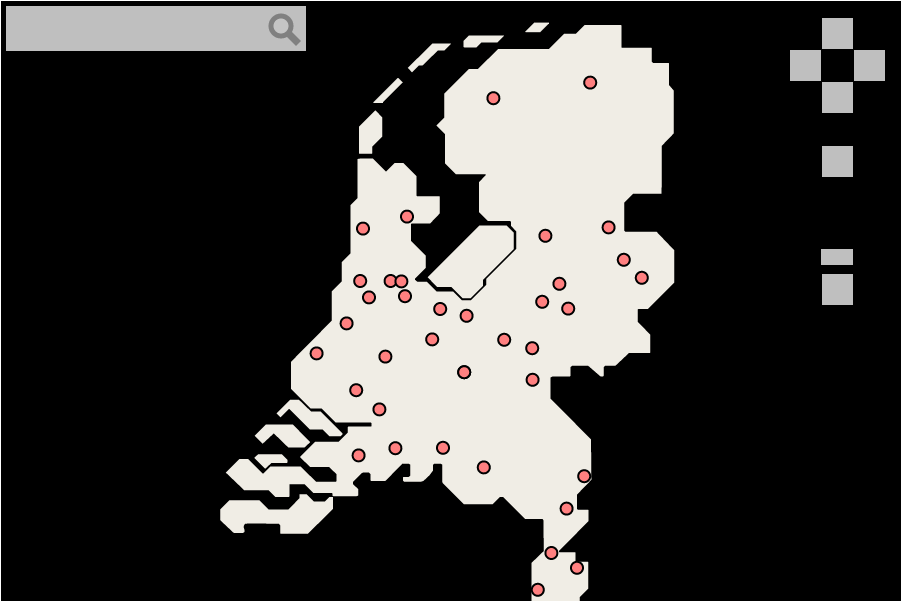
\includegraphics[keepaspectratio,width=\textwidth]{./images/demo.png}
\caption{Een demoapplicatie van de Canvas.hs library}
\label{fig:demo_screenshot}
\end{center}
\end{figure}


\autoref{fig:overzicht_architectuur} geeft een overzicht van de architectuur. Canvas.hs bestaat uit een module en een client. De module is een library die de programmeur in zijn programma importeert. Bij het starten van de module start een HttpServer, een WebSocket-server en wordt de webpagina van de client automatisch gestart. De client bestaat uit een browserpagina met onder andere een canvas element. De module communiceert met de client via een WebSocket verbinding om grafische elementen op de canvas in de client te tekenen.

\begin{figure}[H]
\begin{center}
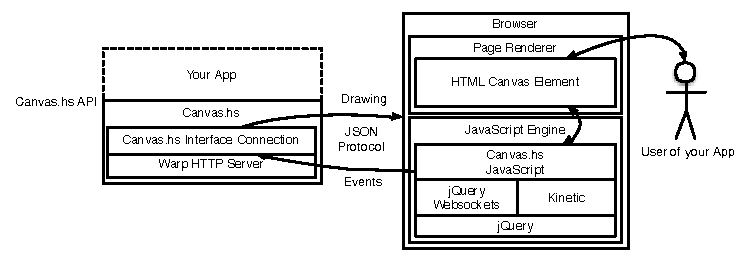
\includegraphics[keepaspectratio,width=\textwidth]{./images/architectuur_overzicht.pdf}
\caption{Overzicht van de architectuur van Canvas.hs}
\label{fig:overzicht_architectuur}
\end{center}
\end{figure}


Voor elke gebeurtenis (event, zoals bijvoorbeeld een muisklik) die binnen het systeem plaatsvindt wordt de code van de user applicatie aangeroepen. Deze eventHandler kan op basis van deze gebeurtenis een nieuwe grafische boom opleveren, hierbij kan gedacht worden aan een boom met daarin o.a. text en simpele vormen die samen een groter geheel vormen. Dit wordt hieronder toegelicht in \autoref{par:globaal_shapes}. Deze boom zal vervolgens op het canvas getekend worden. 

De eventhandler kan daarnaast ook nog een aantal uit te voeren acties opleveren, hierbij kan gedacht worden aan bijvoorbeeld het lezen of schrijven van bestanden. 

Daarnaast heeft de eventHandler de mogelijkheid om state bij te houden. Elke keer dat deze door Canvas.hs wordt aangeroepen krijgt deze de vorige opgeleverde state mee en de eventhandler heeft een nieuwe state in het resultaat. 

Het type van de eventHandler ligt bovenstaande duidelijk toe: \inlinecode{eventHandler :: a -> Event -> (a, Output)}, hierin is \inlinecode{a} de state die de eventHandler kan bijhouden. \inlinecode{Output} is een datatype waarin acties en een grafische boom gecombineerd kunnen worden.


\autoref{eventHandler_voorbeeld_simpel} illustreeert een simpele eventHandler die bij de start van het programma (\inlinecode{StartEvent}) een vierkant tekent en een timer start. Vervolgens wordt elke keer dat deze Timer afgaat het vierkant verplaatst. Als state wordt een simpele \inlinecode{Int} gebruikt. D.m.v de installEventHandler functie van Canvas.hs wordt de eventHandler geregistreerd en het systeem gestart.

\begin{lstlisting}[caption=Voorbeeld van een simpele eventHandler, label=eventHandler_voorbeeld_simpel]
import CanvasHs
import CanvasHs.Data

type State = Int

main = installEventHandler handle 0

handle :: State -> Event -> (State, Output)
handle st StartEvent    = (st+1, output)
	where 
		output = Out (Just shape, actions)
		shape = rectangle st
		actions = [Timer 1000 "move"]
		
handle st (Tick "move") = (st+1, shape $ rectangle st)
		
rectangle :: State -> Shape
rectangle i = Rect (10*i, 10*i) 10 10
\end{lstlisting}

Een gedetailleerde handleiding over Events, Shapes, Actions in het algemeen het gebruik van Canvas.hs kan gevonden worden in \autoref{sec:gebruikershandleiding}: gebruikerhandleiding.

\paragraph{Shapes}
\label{par:globaal_shapes}
Zoals hierboven aangegeven levert de eventHandler o.a. een grafische boom op. Deze boom is gebasseerd op het Shapetype. Dit type definieert een aantal primitieven, zoals lijnen en vierkanten, en aantal translaties zoals verschuivingen en rotaties die op een primitieve worden toegepast. Daarnaast wordt via het Shapetype ook aangegeven of er interesse is in events, zoals muiklikken, die plaatsheben op de Shape. In \autoref{dia:grafische_boom} is een grafische boom van Shapes weergegeven. Zoals te zien bestaan de bladen van de boom altijd uit primitieven en hebben de translaties altijd één Shape als subboom.

\begin{diagram}
\Tree [.Container [.Fill [.Rotate [.{Event mouseClick=True} Rect ] ] ] [.Translate Text ] [.Stroke [.Container [.Circle ] [.Line ] [.Circle ] ] ] ]
\caption{Grafische boom}
\label{dia:grafische_boom}
\end{diagram}

\paragraph{Communicatie}
In Canvas.hs wordt de grafische weergave gedaan door het canvaselement in een webbrowser. Voor de communicatie tussen het haskellprocess en de webbrowser zijn een aantal mogelijkheden. In Canvas.hs hebben we ervoor gekozen in het Haskellprocess een server te starten die vervolgens door de webbrowser wordt aangesproken. Hier wordt over uitgeweid onder \autoref{subsec:architectuur}: architectuur.

\paragraph{Externe bibliotheken}
Voor het opzetten van deze server zijn vele oplossingen bedacht in de vorm van modules voor Haskell. Ook voor de interactie met het canvaselement bestaan een aantal JavaScriptbibliotheken.
In Canvas.hs hebben wij het wiel niet opnieuw uitgevonden, maar de beste van deze oplossingen geselecteerd. De gekozen bibliotheken worden verder toegelicht onder \autoref{subsec:externe_libraries}: externe bibliotheken.
